\documentclass{beamer}
\usetheme{afm}

\title{Arbitrage-Free Pricing Theory}
\subtitle{Let's refresh some useful concept}
\course{Advanced Financial Modelling}
\author{\href{mailto:matteo.sani@unisi.it}{Matteo Sani}}

\begin{document}
	\begin{frame}[plain]
		\maketitle
	\end{frame}        

%\begin{frame}{}
%\begin{block}{Disclaimer}	
%Concerning this part I am assuming that:
%\begin{itemize}
%\item you know what is a random process;
%\item you know what is a stochastic differential equation (SDE);
%\item you know a bit of stochastic calculus (Ito's lemma, Ito's %integral\ldots);
%\item you know (or have heard of) no-arbitrage pricing theorems;
%\item you know (or have heard of) Monte Carlo Simulation.
%\end{itemize}
%\end{block}
%\end{frame}	


\section{Stochastic Calculus}
\subsection{Stochastic Processes}
\begin{frame}{Random Variables}
	\begin{block}{Definition}
	A variable whose value is a number determined by the outcome of a random experiment is called a \textcolor{red}{random variable}.
	
	It is a mapping between 
	\begin{equation*}
		X(\omega):\Omega\rightarrow \mathbb{R}\quad \forall\omega\in\Omega
	\end{equation*}
	such that $X(\omega)$ represents the occurrence probability of the "outcome" $\omega$. $\Omega$ is called \textcolor{red}{sample space} and is the set of all possible future states (or outcomes) of the random process.
	\end{block}
        
	If $X$ represents the outcomes of rolling a \emph{fair} die $\Omega = [1,2,3,4,5,6]$ and each value has equal probability of 1/6.
	\vspace{0.5cm}
        
	\textcolor{red}{A random variable is always associated to a probability distribution.}
\end{frame}

\begin{frame}{Characterizing a Random Variable}
	We can characterize it by a couple of numbers (\emph{statistics}).
	\small{
		\begin{center}
			\textcolor{red}{mean:} $\boxed{\mu = \mathbb{E}[X] = \int_{-\infty}^{\infty} xf(x)dx}$\quad
			\textcolor{red}{variance:}  
			$\boxed{\sigma^2 = \mathbb{E}[(X-\mu)^2] =\int_{-\infty}^{\infty} (x-\mu)^2f(x)dx}$
	\end{center}
}
	\renewcommand{\arraystretch}{1.4}
{\tiny {\tiny }}{
	\begin{table}[bt]
		\begin{tabular}{|c|c|} \hline
			Scalar multiplication & $\mathbb{E}[aX] = a\mathbb{E}[X]$ \\ \hline
			Sums & $\mathbb{E}[X_1+\ldots +X_K] =  \mathbb{E}[X_1] +\ldots + \mathbb{E}[X_n]$ \\ \hline
			Linear combinations & $\mathbb{E}[a_1X_1+\ldots +a_KX_K] =  a_1\mathbb{E}[X_1] +\ldots + a_K\mathbb{E}[X_K]$ \\ \hline
			Expected value of a constant & $\mathbb{E}[a] = a$ \\ \hline
			Products (independent variables) & $\mathbb{E}[XY] = \mathbb{E}[X] \mathbb{E}[Y]$ \\ \hline
		\end{tabular}
	\end{table}
}
Essentially all the expectation properties come from integration properties,
\end{frame}

\begin{frame}{Stochastic Differential Equation}
\begin{block}{Definition}
A collection of random variables that is indexed by some mathematical set (usually time) is called a \textcolor{red}{stochastic processes}.
\end{block}
Stochastic processes are described by \emph{stochastic differential equations} (SDE):	
	\begin{equation}
		\begin{aligned}
			dX(t) = \mu(t,X(t)) dt &+ \sigma(t,X(t)) dW(t) =\\  & =\underbrace{\mu(t,X(t))dt}_{\textrm{deterministic}} + \underbrace{\sigma(t,X(t)) \mathcal{N}(0,1)\sqrt{dt}}_{\textrm{stochastic}}
		\end{aligned}
	\label{eq:sde}
	\end{equation}
	
\begin{itemize}
\item $W(t)$ is called a \emph{Wiener Process}, is normally distributed and independent of everything has happened up to time $t$;
\item for $s< t$ the stochastic variable $W(t)-W(s)$ has a Gaussian distribution $\mathcal{N}(0, t)$, i.e. the standard deviation grows with the square root of time.
\end{itemize}  
\end{frame}

\begin{frame}{Wiener Process}
	\begin{itemize}
		\item Using simple properties of the normal distribution we can obtain the following results:
			\begin{equation*}
				\begin{gathered}
					\mathbb{E}[\Delta W] = 0 \\
					\Cline[red]{\mathbb{E}[(\Delta W)^2] = \Delta t} \\
					\text{Var}[\Delta W] = \Delta t \\
					\Cline[red]{\text{Var}[(\Delta W)^2] = 2(\Delta t)^2} \\
				\end{gathered}
			\end{equation*}
		\item The striking fact is that as $\Delta t$ tends to 0, $[(\Delta W)^2]$ goes to 0, but its variance will approach 0 much faster.
		\item Thus, heuristically, we can say that $[(\Delta W)^2]$ looks more and more "deterministic", and in the limit we can naively say:
		\begin{equation*}
		\boxed{dW^2 = dt}
		\end{equation*}
	\end{itemize}
\end{frame}

\begin{frame}{Stochastic Integral}
	\begin{itemize}
		\item It is possible to interpret~\cref{eq:sde} as a shorthand for 
			\begin{equation*}
				X(t) = X(0) + \int_0^t \mu(s,X(s)) ds + \int_0^t \sigma(s,X(s)) dW(s)
			\end{equation*}
		where the last term is the so-called \emph{It$\hat{o}$'s integral}.
		\item Without entering into the details of stochastic calculus we can state the two most important properties of an It$\hat{o}$ integral:
			\begin{equation*}
				\begin{gathered}
					\mathbb{E}\left[\int_a^b g(s) dW(s)\right] = 0 \\
					\mathbb{E}\left[\left(\int_a^b g(s) dW(s)\right)^2\right] = \int_a^b\mathbb{E}[g^2(s)]ds\\
				\end{gathered}
			\end{equation*}
	\end{itemize}  
\end{frame}

\begin{frame}{Filtration}
	\begin{block}{Definition}
		With the symbol $\mathcal{F}^X_t$ it is indicated a \textbf{filtration}. It represents the information generated by $X$ in the interval $[0, t]$, i.e. what has happened to $X$ over the interval. 
	\end{block}
	\begin{itemize}	
		\item If the value of a stochastic variable $X$ ca be completely determined given observations of its trajectories $\{X(s); 0\leq s \leq t\}$, then we can write $X\in\mathcal{F}_t^X$ and $X$ is said to be $\mathcal{F}_t^X$\emph{-measurable}.
		\item If $Y$ is a stochastic process such that $Y(t)\in\mathcal{F}_t^X$ for all $t$ then we say that $Y$ is \emph{adapted} to the filtration $\mathcal{F}_t^X$. 
	\end{itemize}
\end{frame}

\begin{frame}{Conditional Expectation}
	\begin{block}{Definition}
		Given the information (filtration) $\mathcal{F}_t$, for any stochastic variable $X$ consider
		\begin{equation*}
			\mathbb{E}[X|\mathcal{F}_t]
		\end{equation*}
		which represents the \textbf{conditional expectation} of $X$.
		%By definition it also holds that $\mathbb{E [\mathbb{1}_{\mathcal{F}}X] = \mathbb{E}[\mathbb{1}_{\mathcal{F}}\mathbb{E}[X|\mathcal{F}]]$.
	\end{block}
	\begin{itemize}
		\item Given $X$ and $Y$ stochastic variables with $Y$ $\mathcal{F}_t$-measurable:
		\begin{equation*}
			\mathbb{E}[Y\cdot X|\mathcal{F}_t] =  Y\cdot\mathbb[X|\mathcal{F}_t]
		\end{equation*}
		indeed if $Y\in\mathcal{F}_t$ we know exactly its value, so in the expectation it can be treated as a constant and taken outside.
	\end{itemize}
\end{frame}

\begin{frame}{Martingale}
	\begin{block}{Definition}
		A \textcolor{red}{martingale} is a stochastic process which models a fair game with the following remarkable feature
		\begin{equation}
			\mathbb{E}[X_t|\mathcal{F}_s] = X_s
		\end{equation}
		so the best prediction for the future value $X_t$, given the knowledge $\mathcal{F}_s$ at time $s$ is the value at time $s$ itself, $X_s$.
	\end{block}
%	\begin{block}{Properties}
	\begin{itemize}
	\item If $X_t$ is a stochastic process with diffusion coefficient $\sigma_t$, such that %which satisfies $\mathbb{E}\left[\left(\int_0^T\sigma^2_s ds\right)^{\frac{1}{2}}\right]<\infty$, and SDE 
	$dX_t=\mu_t dt+\sigma_t dW_t$, then 
	\begin{equation*}
		X\text{ is a martingale } \iff X\text{ is drift-less } (\mu_t=0)
	\end{equation*}
	\item A martingale corresponds to the common notion that "a price, changes randomly" so we cannot know if it will go up or down.
\end{itemize}
\end{frame}
	
\section{No Arbitrage Theory}
\subsection{No Arbitrage Principle\ldots}

\begin{frame}{Risk Neutral Pricing Foundations}
	Harrison and Pliska proved and formalized the following results:
	\begin{itemize}
		\item \textbf{The market is free of arbitrage if (and only if) there exists an \textcolor{red}{equivalent martingale measure} (EMM) (i.e. a risk-neutral measure).}
	\end{itemize}
	\vfill
\end{frame}

\begin{frame}{Risk Neutral Pricing Foundations}
	\begin{itemize}
		\item Arbitrage opportunities rarely exist in practice. If and when they do, gains are extremely small, and are typically short-lived and difficult to spot. \textcolor{red}{Arbitrage exclusion in the mathematical model is close enough to reality}.
		\item An \textcolor{red}{equivalent martingale measure} $\mathbb{Q}$ is a probability measure on the space $\Omega$ such that
		\begin{enumerate}
			\item $\mathbb{Q}$ is equivalent to $\mathbb{P}$ (real world measure);
			\item for any asset $A$ and for each time $t$, $0\le t\le T$ there exists a (martingale) price $\pi_t$
			\begin{equation*}
				\pi_t = \expect{Q}[D(t,T)V_A|\mathcal{F}_t]
			\end{equation*}
		\end{enumerate}
	\end{itemize}
    \begin{block}{Definition}
    A \textbf{(probability) measure} ($\mathbb{P}, \mathbb{Q}\ldots$) is a mapping which associates a probability to each element in the sample space. Two measures are \textbf{equivalent} if they agree "on what is possible". Note the word \emph{possible}: the two measures can have different probabilities for the same event, but must have the same \emph{null-set} $\{x\in {\mathbb{P}}\mid p (x)=0\}$.
    \end{block}
\end{frame}

\subsection{Risk Neutral Measure}
\begin{frame}{Risk Neutral Measure}
\begin{itemize}
\item  The difference between real world and risk neutral measures is in the treatment of the market price of risk.
\item If you tried to estimate the anticipated value of a stock based on how likely it is to go up or down, considering unique factors or market conditions that influence that specific asset, you would be including risk into the equation and, thus, would be looking at \textcolor{red}{real or physical probability}.
\item The \textcolor{red}{risk neutral measure}, instead, allows determination of a market-consistent value without making any assumption about the market price of risk. That is useful because the price of risk is not directly observable, but the market prices used to calibrate a risk-neutral generator are.
\item The risk neutral measure is a direct consequence of no arbitrage assumption. It is an \emph{implied probability distribution} from observable prices of tradable instruments, and used to determine \textcolor{red}{objective fair prices} for a financial instrument.
\end{itemize}
\end{frame}

\begin{frame}{Risk Neutral Pricing Foundations}
	Harrison and Pliska proved and formalized the following results:
	\begin{itemize}
		\item The market is free of arbitrage if (and only if) there exists an \textcolor{red}{equivalent martingale measure} (EMM) (i.e. a risk neutral measure).
		\item \textbf{The market is complete if and only if the martingale measure is unique.}
		
		(Note that market completeness means that any contingent claim can be replicated by a portfolio, or in other words that every asset in every possible state of the world has a price.)
	\end{itemize}
    \begin{block}{Definition}
		A \textbf{contingent claim} is a contract whose future payoff depends on the value of another “underlying” asset, or more generally, that is dependent on the realization of some uncertain future event $(S, X\ldots)$		    
	\end{block}
    \vfill
\end{frame}

%\begin{frame}{Summary of Basic Definitions}
%	\begin{itemize}
%		\item The market is complete if and only if the martingale measure is unique.
%		\item In a complete and arbitrage-free market the price of any derivative is uniquely given, either by the value of the associated replicating strategy, or by the expectation of the discounted payoff under the risk-neutral measure
%		\begin{equation}
%			\Pi_t = \mathbb{E}^{\mathcal{Q}^0}[D(t,T)V_A|\mathcal{F}_t]
%			\label{eq:risk_neutral_pricing}
%		\end{equation}
%	\end{itemize}
%\end{frame}

\begin{frame}{Risk Neutral Pricing Foundations}
	Harrison and Pliska proved and formalized the following results:
	\begin{itemize}
		\item The market is free of arbitrage if (and only if) there exists an \textcolor{red}{equivalent martingale measure} (EMM) (i.e. a risk-neutral measure).
		\item The market is complete if and only if the martingale measure is unique;
		\item \textbf{In a complete and arbitrage-free market the price of any derivative is uniquely given, either by the value of the associated replicating strategy, or by the expectation of the discounted payoff under the risk-neutral measure}
		\begin{equation}
			\Pi_t = \expect{Q}[D(t,T)V_A|\mathcal{F}_t]
			\label{eq:risk_neutral_pricing}
		\end{equation}
	\end{itemize}
\end{frame}

\section{Monte Carlo Simulation}
\subsection{The Technique}
\begin{frame}{What is a Monte Carlo Simulation ?}
\begin{itemize}
	\item Our main goal is to compute prices with \cref{eq:risk_neutral_pricing}, which may not always be analytically solvable.
	\item In addition, many stochastic factors (stock prices, interest rates\ldots), influence the result, making predictions challenging. 
	\item \textbf{The Monte Carlo simulation technique} is the right tool to tackle this kind of  problems.
	\item It is a probability-based simulation method that uses random sampling to analyse uncertain outcomes.
	\item Instead of relying on single point estimates, \emph{it generates multiple scenarios based on probability distributions}. 
	\item This allows to assess the range of potential outcomes providing a more comprehensive understanding of the problem in hand.
\end{itemize}
\end{frame}

\begin{frame}{Monte Carlo in Practice}
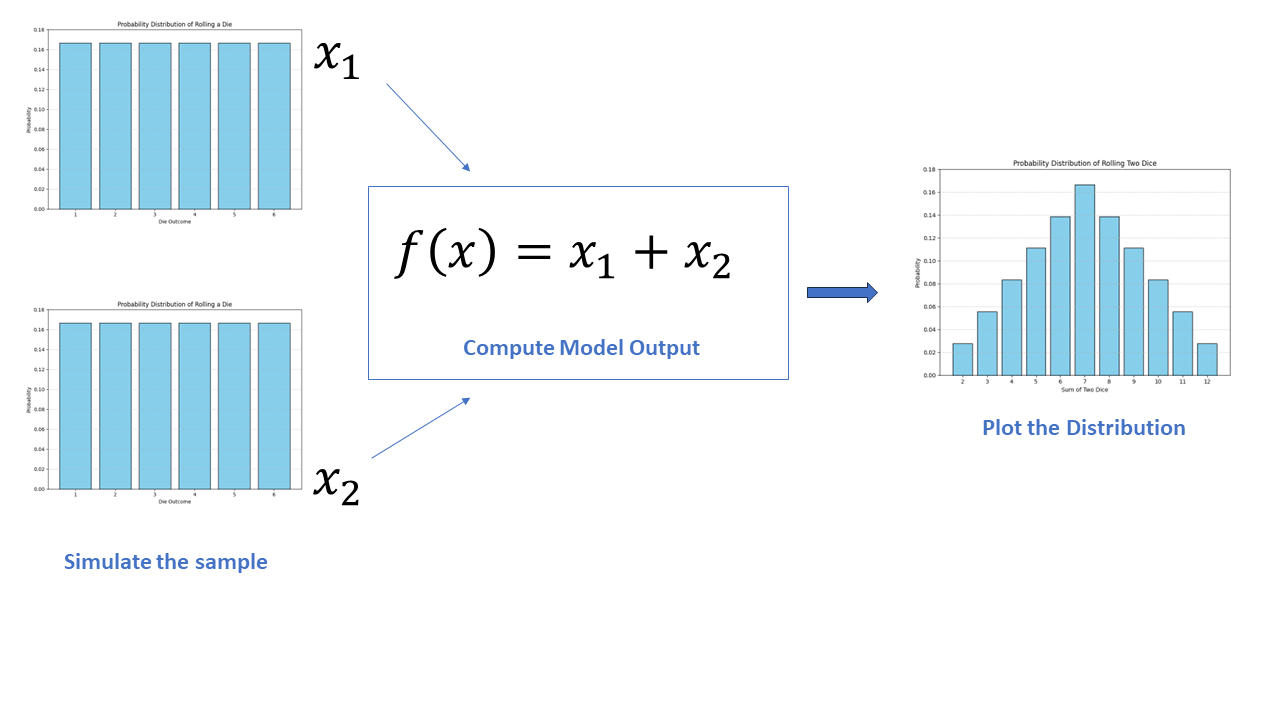
\includegraphics[width=1.0\linewidth]{images/monte_carlo_simulation}
\end{frame}

\begin{frame}[fragile]{Monte Carlo in Practice}
\begin{columns}
	\column{0.5\linewidth}
\begin{ipython}
import numpy as np
import matplotlib.pyplot as plt

num_trials = 10000

sums = []
for _ in range(num_trials):
    rolls = np.random.randint(1, 7, size=2)
    total_sum = np.sum(rolls)
    sums.append(total_sum)
\end{ipython}
    \column{0.5\linewidth}
    \begin{center}
    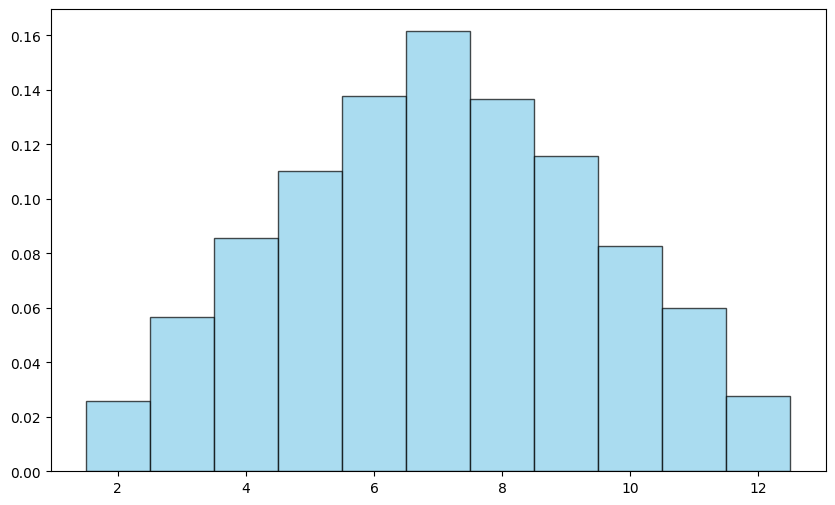
\includegraphics[width=0.8\linewidth]{images/sum_two_dice}
    \end{center}
\end{columns}
\end{frame}

\subsection{Central Limit Theorem}
\begin{frame}{Central Limit Theorem}
\begin{itemize}
\item The \emph{population} is the entire dataset collected based on common characteristics which can be used for statistical purposes.
\item The \emph{sample} is a subset of a population with fewer data points i.e. data selected randomly from a population.
\end{itemize}
\begin{block}{Theorem}
The \textbf{Central Limit Theorem} states: \emph{the sampling distribution of the mean is normally distributed, as long as the sample size is large enough}.
	
\begin{enumerate}
    \item the best estimate of a quantity given by MC experiments is the \textbf{mean} of the simulation results;
    \item with a larger sample size, your sample mean is \textbf{more likely to be close to the population mean} (more precise estimate).
\end{enumerate}
\end{block}
\end{frame}

\begin{frame}[fragile]{Central Limit Theorem Example}
\begin{columns}
    \column{0.5\linewidth}
         \begin{table}
            \centering
            \begin{tabular}{cc}
                Size & Estimated Mean \\
                \hline
                10 & $7.046 \pm 0.763$\\
                50 & $7.026 \pm 0.334$ \\
                500 & $7.006 \pm 0.103$ \\
            \end{tabular}
            \label{tab:my_label}
        \end{table}
    \column{0.5\linewidth}
        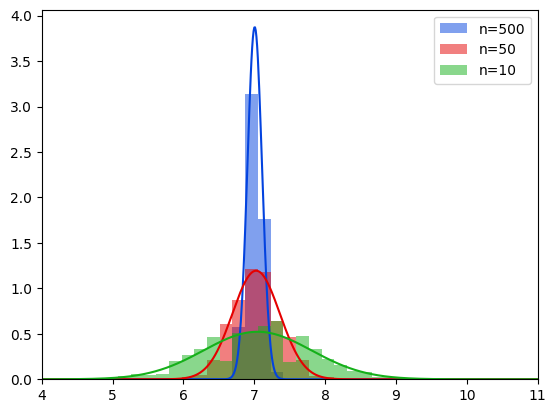
\includegraphics[width=0.8\linewidth]{images/sample_mean}
\end{columns}
\begin{itemize}
    \item The resulting "improvement" can also be quantified:
    \begin{equation}
    \cfrac{0.103}{0.334} = 0.308 \simeq \sqrt{\cfrac{50}{500}} = 0.316
    \label{eq:clt}
    \end{equation}
    which tells us that \textbf{the uncertainty scales as the square root of the sample size}.
\end{itemize}
\end{frame}

\begin{frame}{Central Limit Theorem Example}
\begin{itemize}
    \item This shows that no matter what our population distribution curve is, the sample means will always follow Gaussian Distribution.
    \item Sample sizes equal to or greater than 30 are considered sufficient for the theorem to hold but that might not be always necessary. In our example, we can observe that we get a Gaussian Distribution with a sample size of 10 or 20 too.
    \item Statistical analysis of the data of the entire population are practically impossible in almost all cases. Sample data of any population can be used to draw conclusions about the overall population using CTL as we know that sample means are always normally distributed!!!!
\end{itemize}
\end{frame}

\subsection{Monte Carlo Applications}
\begin{frame}{Stochastic Simulation}
\begin{itemize}
    \item Consider a generic SDE of the form  
        \begin{equation*}
        dX(t) = \mu(t,X(t))dt + \sigma(t,X(t))dW(t) 
        \end{equation*}
    \item The simulation of $X(t)$ follows the \emph{Euler Scheme}: starting from the \textbf{known} value of $X(t_0)$ simply compute $X(t_0 +\Delta t)$ using the given SDE:
        \begin{equation*}
            X(t_0+\Delta t) = X(t_0) + dX(t)
        \end{equation*}
    \item Setting $\Delta t$ to a "reasonable" value, $dX$ can be computed by evaluating the two coefficients $\mu(t_0,X(t_0))$ and $\sigma(t_0,X(t_0))$; $dW$ is a standard Brownian motion, so its value can be obtained by sampling from a standard normal $Z=\mathcal{N}(0,1)$:
        \begin{equation*}
            X(t_{i+1}) = X(t_i) + \mu(t_i,X(t_i))\Delta t + \sigma(t_i,X(t_i))\sqrt{\Delta t}Z 
        \end{equation*}
    \end{itemize}
\end{frame}

\begin{frame}[fragile]{Brownian Motion Example}

In the specific case of a simple Brownian motion the dynamics is given by $dW = \sqrt{dt}\mathcal{N}(0,1)$ so
\begin{equation}
W(t+\Delta t) = W(t) + \sqrt{\Delta t}Z \implies
W(t) = W(t_0) + \sum_{t_0}^{t} \sqrt{\Delta t}Z
\label{eq:bm_evolution}
\end{equation}

\begin{block}{\texttt{Python} Digression}
For the rest of the course we are going to show \texttt{python} examples using a framework we have developed, mostly hiding the underlying technical details.

For the BM example, I would like to show how usually this problems are tackled in \texttt{python} analysing, once and for all, the code.
\end{block}
\end{frame}

\begin{frame}{Brownian Motion Example}
\begin{itemize}
    \item \texttt{Python} is not that great when dealing with complex calculation; the trick that is usually used in these cases is to move to \emph{linear algebra} using dedicated libraries which are highly optimized for such calculations (e.g. \texttt{numpy}).
    \item The goal here is to simulate $N$ \emph{realizations} of a Brownian motion (BM) process with $m$ \textit{time steps} and initial value 0. 
    \item Instead of performing each single calculation for each time step and each realization, we are going to use matrices and perform bunch of operations at once.
    \item Let's start with a $(N\times m)$ matrix $[W_0]$
    $$
    [W_0] =
    \begin{bmatrix}
    W^1_0 & W^2_0 & \cdots & W^N_0 \\
    0 & 0 & \cdots & 0 \\
     &  & \vdots &   \\
    0 & 0 & \cdots & 0 \\
    \end{bmatrix}
    $$
    \end{itemize}
\end{frame}

\begin{frame}{Brownian Motion Example}
\begin{itemize}
    \item Then we calculate each variation by sampling $N\times (m-1)$ times from the Normal distribution and create a second matrix 
    $$
    [dW] =
    \begin{bmatrix}
    0 & 0 & \cdots & 0 \\
    dW^1_1 & dW^2_1 & \cdots & dW^N_1 \\
     &  & \vdots &   \\
    dW^1_{m} & dW^2_{m} & \cdots & dW^N_{m} \\
    \end{bmatrix}
    $$  
    \item Let's sum 
    $$[W] = [W_0] + [dW] =
    \begin{bmatrix}
    W^1_0 & W^2_0 & \cdots & W^N_0 \\
    dW^1_1 & dW^2_1 & \cdots & dW^N_1 \\
     &  & \vdots &   \\
    dW^1_{m} & dW^2_{m} & \cdots & dW^N_{m} \\
    \end{bmatrix}
    $$  
\end{itemize}
\end{frame}

\begin{frame}{Brownian Motion Example}
\begin{itemize}
    \item Finally, remembering \cref{eq:bm_evolution}, we can obtain the Brownian motion evolution in each realization by simply summing up all the columns in $[W]$

\[\left[
\begin{array}{cccc}
W^1_0 & W^2_0 & \cdots & W^N_0 \\
\downarrow & \downarrow & \cdots & \downarrow \\
dW^1_1 & dW^2_1 & \cdots & dW^N_1 \\
\downarrow & \downarrow & \vdots & \downarrow \\
dW^1_{m} & dW^2_{m} & \cdots & dW^N_{m} \\
\downarrow & \downarrow & \cdots & \downarrow \\
W^1_0+\sum\limits_{i=1}^{m} dW^1_i & W^2_0+\sum\limits_{i=1}^{m} dW^2_i & \cdots & W^N_0+\sum\limits_{i=1}^{m} dW^N_i
\end{array}\right]
\]
\end{itemize}
\end{frame}

\begin{frame}[fragile]{Brownian Motion Example}
\begin{columns}
	\column{0.55\linewidth}
\begin{ipython}
import numpy as np

N = 10
m = 100
W0 = 0

W = np.zeros(shape=(m, N))
W[0, :] = W0
W[1:, :] = np.random.normal(size=(m-1, N))*np.sqrt(1/m)
W = np.cumsum(W, axis=0)
\end{ipython}
    \column{0.4\linewidth}
\begin{center}    
    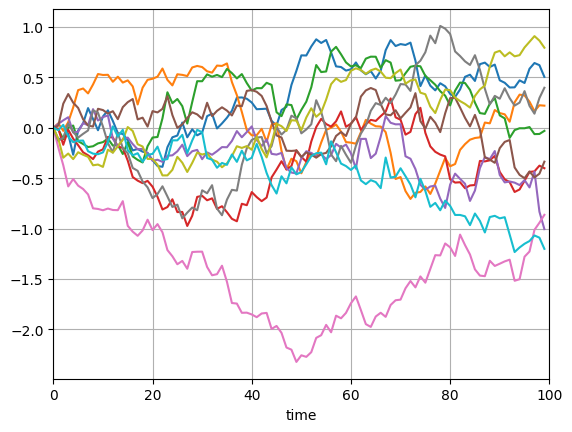
\includegraphics[width=1.\linewidth]{images/bm_realizations}
\end{center}
\end{columns}
\begin{block}{Important}
Those are just 10 \emph{possible} realizations of a  BM: as a stochastic process it is impossible to know how it will develop in the future. A statistical analysis of a stochastic process necessarily involves to average ($\mathbb{E}$) among the possible paths.
\end{block}
\end{frame}

\begin{frame}{Geometric Brownian Motion Example}
\begin{itemize}
    \item Similarly to what have been done before we can simulate the evolution of a Geometric Brownian Motion (GBM), the random process that usually models stocks
    \begin{equation*}
        dS(t) = \mu S(t) dt + \sigma S(t) dW(t)
    \end{equation*}
    where: $\mu$ is the drift term (expected return), $\sigma$ is the volatility (standard deviation of the returns), and $dW$ is a standard Wiener process (Brownian motion).
    \item The proceed we can either implement again the Euler scheme or directly use the analytical solution of the GBM
    \begin{equation*}
        S(t) = S(0)e^{(\mu-\frac{1}{2}\sigma^2)t+\sigma W_t}
    \end{equation*}
    where $S_0$ is the initial price of the asset at time.
    %\item Notice that the logarithm of $S(t)$ follows a normal distribution:
    %\begin{equation*}
    %    \ln(S(t)) = \mathcal{N}\left(\left[\ln(0) +\left(\mu +\cfrac{\sigma^2}{2}\right)t \right], \sigma^2 t\right)
    %\end{equation*}
\end{itemize}
\end{frame}

\begin{frame}[fragile]{Geometric Brownian Motion Example}
\begin{itemize}
    \item Let's see the results of such a simulation for a 8-months (with daily steps) period with initial value $S_0=100$, $\mu=0.005$, and $\sigma=0.05$.
\end{itemize}

\begin{columns}
	\column{0.55\linewidth}
\begin{ipython}
import tensorquant as tq
import tensorflow as tf

gbm = tq.GeometricBrownianMotion(mu=0.005, sigma=0.05, x0=100)

n_path = 10
timesteps = 240
Z = tf.random.normal((n_path, timesteps), seed=12, 
                     dtype=tf.dtypes.float64)
t = tf.Variable(8, dtype=tf.float64)
S_t = gbm.evolve(t, Z)    
\end{ipython}
    \column{0.4\linewidth}
\begin{center}    
    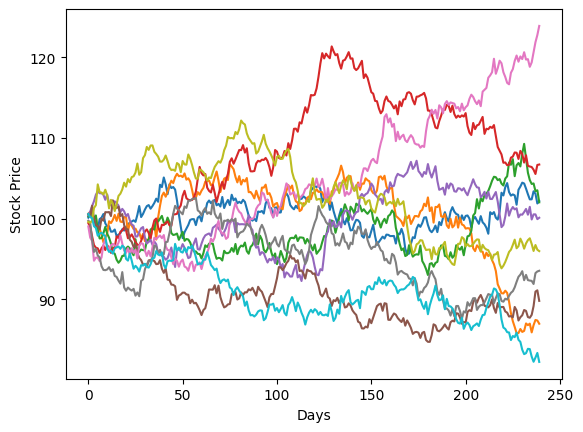
\includegraphics[width=1.1\linewidth]{images/gbm_realizations}
\end{center}
\end{columns}
%If you want to try this code remember to install \texttt{tensorquant} with the command \texttt{pip install tensorquant}.
\end{frame}

\begin{homework}
\begin{frame}{\textcolor{white}{Homework}}
\begin{itemize}
\item[white]  You have determined the value of an interest rate derivative with a Monte Carlo simulation involving 50 scenarios which results in a contract value of 1.2 M€ $\pm$ 5\%. Unfortunately, your boss asks you to determine more precisely the derivative value. If you have to meet him in 1 hour and each simulation lasts about 2.5 sec., what is the highest precision you can achieve ?
\item[white] Consider the process $Y(t) = 2^{W(t)}$, where $\{W(T):t\geq 0\}$ is a standard Brownian motion. Is this a martingale ?
\item[white]  Show that the exponential SDE
\begin{equation*}
dX_t = A_t X_tdW_t,\quad X_0=x_0
\end{equation*}
has the following solution
\begin{equation*}
X_t = x_0 e^{-\frac{1}{2}\int_0^t A_0^2 ds+\int_0^t A_s dB_s}
\end{equation*}
\end{itemize}
\textcolor{white}{Exercises for this part involves: SDE solving, martingale definition, Ito's lemma, and a bit of Monte Carlo theory.}
\end{frame}
\end{homework}

\section{Backup}

\begin{frame}{Probability Distribution}
	Let $X$ be a random variable defined on a domain $\Omega$ of possible outcomes. 
	\renewcommand{\arraystretch}{1.6}
	\begin{table}[bt]
		\begin{tabular}{|c|c|} \hline
			\textbf{Discrete} & \textbf{Continuous} \\ \hline
			Probability Mass & Probability Density \\ \hline		
			$P(X=x_i)\;\forall x_i\in\Omega$ & $P(X=x)=\int_x^{x+dx}f(x)dx$ \\ \hline
			$P(x_i) \geq 0;\;\forall i$ & $f(x) \geq 0;\;-\infty < x < \infty$\\ \hline
			$\sum_{i=0}^{n} P_i = 1$ & $\int_{-\infty}^{\infty} f(x) dx = 1$\\ \hline
			\multicolumn{2}{|c|}{Cumulative Distribution} \\ \hline
			$F(x_i) = P(X<x_i) = \sum_{x<x_i} P(x)$ & $F(x) = P(X<a) = \int_{-\infty}^{a} f(x) dx$ \\ \hline
		\end{tabular}
	\end{table}
\end{frame}

\begin{frame}{Geometric Brownian Motion}
	\begin{itemize}
		\item Trade random fluctuations deviate a stock price $S_t$ from a steady state.
		\item The price relative change in $dt$ can be decomposed into two parts
		\begin{itemize}
			\item \textcolor{red}{deterministic}: the expected return from holding the stock during $dt$. It can be expressed as $\mu S_tdt$ (with $\mu$ being the expected rate of return);
			\item \textcolor{red}{stochastic}: models the random changes of the market. A reasonable assumption is to equal this term to $\sigma S_t dW_t$. 
		\end{itemize}
		\item Putting all together, the resulting SDE is
		\begin{equation}
			\begin{gathered}
				dS_t = \mu S_t dt + \sigma S_t dW_t \\
				\frac{dS_t}{S_t} = d\log(S_t) = \mu dt + \sigma dW_t
			\end{gathered}
			\label{eq:log_normal_sde}
		\end{equation}
	\end{itemize}
\end{frame}

\begin{frame}{Interlude: It$\hat{o}$'s Formula}
	\begin{block}{Proposition}
		For any given continuous and differentiable function $G(S,t)$ where S satisfies $dS=adt + bdW_t$, holds
		\begin{equation}
			dG = \left(a\frac{\partial G}{\partial S} + \frac{\partial G}{\partial t} + \underbrace{\frac{1}{2}b^2\frac{\partial^2 G}{\partial S^2}}_{\text{additional term}}\right)dt + b\frac{\partial G}{\partial S} dW
			\label{eq:itos_lemma}
		\end{equation}

	This is essentially an extension of the \emph{Taylor series} for stochastic functions, in the expansion an extra term appears.	
	\end{block}	
\end{frame}

\begin{frame}{It$\hat{o}$'s Formula "Proof"}
	\begin{itemize}
	\item Suppose $X_t$ is an stochastic process that satisfies the SDE
	\begin{equation*}	
	dX_{t}=\mu _{t}\,dt+\sigma _{t}\,dW_{t}
	\end{equation*}.
	\item If $f(t,x)$ is a twice-differentiable scalar function of $x$, its expansion in a Taylor series is
	\begin{equation*}
	df={\frac {\partial f}{\partial t}}\,dt+{\frac {1}{2}}{\frac {\partial ^{2}f}{\partial t^{2}}}\,dt^{2}+\cdots +{\frac {\partial f}{\partial x}}\,dx+{\frac {1}{2}}{\frac {\partial ^{2}f}{\partial x^{2}}}\,dx^{2}+\cdots
	\end{equation*}
	\item Substituting $X_t$ for $x$ and $dX_t$ with the SDE gives
	\begin{equation*}
		\begin{aligned}
		df&={\frac {\partial f}{\partial t}}\,dt+{\frac {1}{2}}{\frac {\partial ^{2}f}{\partial t^{2}}}\,dt^{2}+\cdots +{\frac {\partial f}{\partial x}}(\mu _{t}\,dt+\sigma _{t}\,dW_{t})+\\
		&+{\frac {1}{2}}{\frac {\partial ^{2}f}{\partial x^{2}}}\left(\mu _{t}^{2}\,dt^{2}+2\mu _{t}\sigma _{t}\,dt\,dW_{t}+\sigma _{t}^{2}\,dW_{t}^{2}\right)+\cdots
		\end{aligned}
	\end{equation*}
\end{itemize}
\end{frame}

\begin{frame}{It$\hat{o}$'s Formula "Proof"}
	\begin{itemize}
	\item Stopping the expansion up to the first order (i.e. neglecting higher order terms in $dt^2$ and in $dt dW_t$), collecting $dt$ and $dW$ terms, and remembering that $dW^2=dt$, we obtain
	\begin{equation*}
		\begin{aligned}
			df&={\frac {\partial f}{\partial t}}\,dt+\cancel{{\frac {1}{2}}{\frac {\partial ^{2}f}{\partial t^{2}}}\,dt^{2}}+\cdots +{\frac {\partial f}{\partial x}}(\mu _{t}\,dt+\sigma _{t}\,dW_{t})+\\
			&+{\frac {1}{2}}{\frac {\partial ^{2}f}{\partial x^{2}}}\left(\cancel{\mu _{t}^{2}\,dt^{2}}+\cancel{2\mu _{t}\sigma _{t}\,dt\,dW_{t}}+\sigma _{t}^{2}\,dW_{t}^{2}\right)+\cdots =\\
			&=\left({\frac {\partial f}{\partial t}}+\mu _{t}{\frac {\partial f}{\partial x}}+{\frac {\sigma _{t}^{2}}{2}}{\frac {\partial ^{2}f}{\partial x^{2}}}\right)dt+\sigma _{t}{\frac {\partial f}{\partial x}}\,dW_{t}
		\end{aligned}
	\end{equation*}
	as required.
\end{itemize}
\end{frame}

\begin{frame}{Geometric Brownian Motion}
	\begin{itemize}
		\item Let's apply this expansion to $G=\log(S_t)$ 
		\begin{equation*}
			\frac{\partial G}{\partial S}=\frac{1}{S_t},\;\frac{\partial G}{\partial t}=0,\;\frac{\partial^2 G}{\partial S^2}=-\frac{1}{S_t^2}
		\end{equation*}
		\item Substituting back into It$\hat{o}$'s lemma \cref{eq:itos_lemma} and taking $a$ and $b$ values from \cref{eq:log_normal_sde}
		\begin{equation*}
			dG = \left(a\frac{\partial G}{\partial S} + \frac{\partial G}{\partial t} + \frac{1}{2}b^2\frac{\partial^2 G}{\partial S^2}\right)dt + b\frac{\partial G}{\partial S} dW
		\end{equation*}
	\end{itemize}
    
	\begin{equation*}
	d(\log S_t) = \left[\mu S_t\frac{1}{S_t} + \frac{1}{2}\sigma^2S_t^2\left(-\frac{1}{S_t^2}\right)\right]dt + \sigma dW
	\end{equation*}
	
	\begin{equation*}
	\log(S_t) - \log(S_{t-1}) = \log\frac{S_t}{S_{t-1}}=\left(\mu - \frac{1}{2}\sigma^2\right)dt + \sigma dW 
	\end{equation*}	
	
	\begin{equation}
	S_t = S_{t-1}\exp\left[\left(\mu-\frac{1}{2}\sigma^2\right)dt + \sigma\mathcal{N}(0,1)\sqrt{dt}\right] 
	\label{eq:lognormal_solution}
	\end{equation}
\end{frame}

\begin{frame}{One Period Model}
Consider a bank-account $B(t)=e^{rt}$ ($r$ denote the risk-free rate) and assume today's stock price to be $S_0$. In one period of time from now, the price could be 
\begin{equation*}
	\begin{cases}
		S_0\cdot u = S_u \quad\text{with a certain probability $p_u$} \\
		S_0\cdot d = S_d \quad\text{with a certain probability $p_d$}\\ 
	\end{cases}, \text{with }(u > d)
\end{equation*}

If we want our simple model to \emph{avoid arbitrage opportunities}, we must impose conditions on $u$ and $d$. 

In case $e^r > u$, I could short the stock in $t_0$ and invest the proceeds $S_0$ into the bank account: in both future states in $t_1$, I could buy the stock back for less than my proceeds 
\begin{equation*}
S_0e^r > S_u > S_d
\end{equation*} Similarly for $e^r < d$\ldots

\begin{equation*}
	\boxed{d\le e^r \le u \implies \text{no arbitrage}}
\end{equation*}
\end{frame}

\begin{frame}{Risk-Neutral Measure}
	\begin{equation*}
		\begin{aligned}
			S_0 &= \frac{S_0(u-d)e^r}{(u-d)e^r} = \frac{S_0(u-d)e^r + (S_0ud - S_0ud)}{(u-d)e^r}=\\
			&= \frac{1}{e^r}\left(\frac{S_0ue^r - S_0ud}{u-d} + \frac{-S_0de^r + S_0ud}{u-d}\right)=\\
			&= \frac{1}{e^r}\left(S_0u\frac{e^r - d}{u-d} + S_0d\frac{u - e^r}{u-d}\right)
		\end{aligned}
	\end{equation*}

	The no arbitrage condition implies the following bounds
	\begin{equation*}
		\boxed{0\le\frac{e^r -d}{u-d}\le 1,\quad 0\le\frac{u - e^r}{u-d}\le 1}
	\end{equation*}

	also
	\begin{equation}
		\boxed{\frac{e^r -d}{u-d} + \frac{u - e^r}{u-d} = 1}
	\label{eq:risk_neutral_probabilities}
	\end{equation}
\end{frame}

\begin{frame}{Risk-Neutral Measure}
	So we can interpret $p_u=\cfrac{e^r -d}{u-d}$ and $p_d=\cfrac{u - e^r}{u-d}$ as a \textcolor{red}{(risk-neutral) measure} ($\mathcal{Q}$).\vspace{0.3cm}
	
	\begin{block}{Definition}
		A \textcolor{red}{probability measure} is a real-valued function that assigns probabilities to a set of events in a sample space that satisfies measure properties such as countable additivity, and assigning value 1 to the entire space.
	\end{block}	

	Rewriting previous expression of $S_0$ in terms of the newly defined probabilities
	\begin{equation}
		S_0 = \frac{S_up_u + S_dp_d}{e^r} = e^{-r}\mathbb{E}^\mathcal{Q}[S_1]
		\label{eq:risk_neutral_price}
	\end{equation}
	
	So the stock price is the discounted stock expectation \emph{under the chosen probability measure} at $t_1$.
\end{frame}

\end{document}
